\documentclass[10pt,a4paper]{article}
\usepackage[margin=50pt]{geometry}
\usepackage[T1]{fontenc}
\usepackage[utf8]{inputenc}
\usepackage{amsmath,amssymb,graphicx,booktabs,array}
\usepackage[unicode,breaklinks=true,colorlinks=true,linkcolor=blue,urlcolor=blue]{hyperref}
\setlength{\parindent}{0pt}
\setlength{\parskip}{6pt}
\setlength{\emergencystretch}{2em}
\setlength{\tabcolsep}{3pt}
\hypersetup{pdftitle={Historical and Conditional Forecasts of Sampled Net-Position Peaks},pdfauthor={}}
\begin{document}
\fontsize{10.5}{14}\selectfont
\begin{center}
{\LARGE\bfseries Historical and Conditional Forecasts of Sampled Net-Position Peaks}\par\vspace{8pt}
{\large Comparisons on an FX record and Treasury position aggregates}\par\vspace{6pt}
Working paper - 22 October 2026
\end{center}
\begin{abstract}
We evaluate established conditional methods for forecasting the maximum absolute source-reported position over the current and next H records. Historical headrooms, reanchored increment scenarios and native peaks are compared with ridge quantile regression and multivariate local quantiles. Chronological validation selects parameters from small fixed menus before the added evaluations; the previously inspected FX interval remains exploratory. On 6,625 FX origins, six-record regression with longer history lowers mean pinball loss by 12.66\% relative to the original historical-headroom rule and 14.77\% relative to a reference with the same history and update schedule. Breaches nevertheless increase from 332 to 376. In a separately specified weekly Treasury-bill position aggregate, the declared six-week regression comparison raises loss by 50.79\% and breaches from 28 to 54 over 277 origins. Short-history regression performs poorly at the longer horizon in both sources. A favorable secondary Treasury neighbor comparison reverses on a fixed sparse grid containing only 12 origins. Performance therefore varies with source, horizon and estimation history. The contribution is an application and model-validation comparison using mature estimators. Aggregation, calendar horizons, estimated-forecast incoherence and downloaded vintages limit transfer. The results establish neither conditional coverage nor gains from changing quotes, hedges, capital or funding decisions.
\end{abstract}
\section*{1. Introduction}
A recorded net position can reach a large magnitude and return toward its starting value before a horizon ends. A forecast of the terminal signed position leaves this intervening exposure unmeasured. We study an upper-quantile report for the largest absolute source-reported position at issue and over the next H records. It answers a passive monitoring question: does any recorded future position exceed the issued level in magnitude? The financial interpretation depends on the measurement process; a sampled netted position does not reconstruct a complete hedged book or a funding requirement.

The empirical question is whether simple historical constructions remain competitive when established conditional methods are fitted directly to this peak response. We compare historical headrooms (F), increment paths reanchored to the current signed position (S), and native historical peaks subject to the current magnitude floor (K). Earlier one-state retrieval is retained as a reference. The added procedures are ridge quantile regression (QR), multivariate nearest-neighbor quantiles (KNN), and a scale-adjusted local variant. Their 33 coordinates include position lags, current magnitude, past increment scales and recorded-clock calendar information. These are established statistical operations, not newly proposed estimators.

All direct training responses must have ended by the actual refit time. Historical controls with matching eligible history and update schedules distinguish part of the estimation-budget difference. Validation selects a small menu separately by source, horizon, history and family; all candidates and references are retained. The original FX evaluation archive had already been inspected. Publicly freezing the added procedures before their execution does not restore an unseen holdout.

The favorable FX primary and adverse Treasury primary must be read together. At H=6, QR using 2,880 completed FX episodes lowers mean loss by 12.66\% against the original rolling 720-episode F rule. It also lowers loss by 14.77\% against F with the same 2,880-episode frozen pool and update schedule. Breach occasions rise from 332 to 376, although mean positive overrun falls. At H=24, long-history QR improves on the old S reference by only 1.83\%, with 531 rather than 287 breaches and more than doubled mean positive overrun. Short-history QR instead performs worse at that horizon.

The separate application uses an official weekly compilation of primary dealers' aggregate Treasury-bill market-value positions. It is a different financial measurement process, not a second individual FX dealer or a known-disjoint institutional panel. Its declared H=6, W=260 QR comparison has 50.79\% higher loss than equal-history F, with 54 versus 28 breaches over 277 origins. All four Treasury QR specifications lose to their own F controls. A secondary H=24 neighbor gain reverses on the fixed sparse grid. Units, histories, horizons, release conventions and revised snapshots remain source specific.

The contribution is a comparison that challenges historical peak constructions with credible conditional competitors and records the limits of transfer. The new competitors change the original FX ranking, while the chosen regression procedure has substantial limitations on another measured position series. Eligible-history matching does not isolate a causal information effect from regularization, function class, local response count or validation selection. Elementary geometry explains construction relationships, not predictive optimality. We claim no new calibration theorem, universal forecasting improvement or operational intervention.

\section*{2. Closest work and established method transfer}
The closest empirical lineage is Wisniewski, Lindsay and Lindsay (2020), who already use nearest-neighbor and other regression engines on this FX source family, with positions over the preceding 24 hours and calendar or trading-session information. Their comparisons include quantile, conformal and normalized-conformal interval forecasts. Chapter 6 of Wisniewski's thesis continues related regularized and normalized endpoint constructions (award year 2024; inspected cover 2023). These precedents rule out first-use claims for conditional regression, lag/calendar features, neighbors or normalization on these records. Exact input-byte equality with the accepted version-2 member is not established.

Our response is a single upper quantile of an absolute multi-record maximum including the observed issue floor. A signed endpoint interval does not determine this peak: identical future-record marginals can yield different maxima when their dependence differs. The earlier paper averages two endpoint-quantile losses; its numbers cannot benchmark this single peak score. We instead refit a selected set of established engines to completed peak/headroom labels and evaluate the same response on common origins. This is not a reproduction of that earlier entire model suite.

Financial path extrema are established risk objects. MaxVaR studies the worst mark-to-market loss before a horizon under a portfolio-value first-passage framework (Boudoukh et al., 2004). Petrunia, Sabetti and Voia (2019, updated Discussion Paper 7) study the largest end-of-day net debit across ACSS participants, followed by block maxima or threshold excesses. Their cross-sectional terminal-debit maximum differs from a single series' future two-sided sampled peak. Neither precedent supports a claim that financial peak forecasting itself is new here.

Regression-quantile loss minimization is classical (Koenker and Bassett, 1978). Biau and Patra (2011) develop sequential quantile prediction with lag-neighbor experts, growing history, truncation and loss-weighted aggregation under stated stationarity, ergodicity and regularity conditions. Our fixed pools and delayed overlapping labels do not inherit that consistency theorem. The ridge and local estimators here constitute a bounded challenge, not the strongest possible conditional-model universe. Quantile forests (Meinshausen, 2006), autoregressive quantiles such as CAViaR (Engle and Manganelli, 2004), sequential predictive conformal inference (Xu and Xie, 2023) and volatility-updated or filtered historical simulation (Hull and White, 1998; Barone-Adesi et al., 1999) remain distinct unexecuted alternatives.

Trajectory bands and financial horizon curves also predate this comparison. Conformalized Adaptive Forecasting of Heterogeneous Trajectories (Zhou, Lindemann and Sesia, 2024, arXiv v2) uses trajectory-level calibration and a cross-trajectory exchangeability premise. Sözen (2026) combines multi-horizon expected-shortfall forecasts, shape constraints and joint calibration. Their responses and assumptions differ from this position peak; an overlapping single archive is not automatically an exchangeable set of trajectories. Chronological slicing or response normalization alone transfers no simultaneous or conditional-coverage conclusion. We report realized loss, breaches and severity without borrowing those guarantees.

The remaining distinction is the measured peak target, known floor, completed-label timing, construction/update controls and separately qualified aggregate application. A changed target or dataset alone is not a new method. The directed source search does not establish exhaustive priority for this exact target-and-data combination. Its evidence and selected reading ranges are documented separately from the experiments.

\section*{3. Sources, target and completed information}
The FX input is the one-hour member of the Net Position Time Series Dataset, version 2: 18,576 records from 5 February 2014 01:00 through 24 January 2017 00:00. Wisniewski et al. (2020) describe aggregate client-flow positions across five liquid currency pairs for one market maker. We use datetime and the signed NetPosUsd scalar, rather than reconstructing raw currency positions, hedge transactions or cash movements. The source has 18,420 one-hour and 155 forty-nine-hour adjacent gaps. We preserve chronology without sorting, removing gap-crossing windows or interpolation. The timezone and historical publication/vintage convention remain unverified.

The Treasury source is the New York Fed Primary Dealer Statistics series PDPOSGS-B, identifying Treasury-bill long positions less short positions. The FR 2004 framework supplies a weekly Wednesday-close, market/fair-value basis. The accepted snapshot has 706 seven-day-spaced records from 3 April 2013 through 7 October 2026, in USD millions. It aggregates reporting dealers and can reflect valuation or reporting-composition changes. It does not identify pure customer order flow or gross exposures. Taking an absolute value after summing signed dealer positions permits cancellation; offsetting dealer positions can leave a small aggregate and large individual magnitudes (see also the aggregation discussion in Duffie et al., 2023).

\[
B_t=|N_t|,\qquad P_{t,H}=\max_{0\le h\le H}|N_{t+h}|,\qquad G_{t,H}=P_{t,H}-B_t\ge0.
\]
The issue record is included, so B is a known response lower bound under the stipulated replay convention. H counts subsequent source records, and unobserved inter-record excursions are excluded. Six or 24 Treasury records span six or 24 weeks in this snapshot; FX calendar durations vary across its gaps. All horizons share the same source-specific evaluation issue origins, not the same final response dates.

\[
r(t)=t_0+d\left\lfloor\frac{t-t_0}{d}\right\rfloor,\qquad\mathcal T_{r,H,W}=\{r-H-W+1,\ldots,r-H\}.
\]
At each refit r, every training origin satisfies i+H\(\le\)r\(\le\)t. The transform, response scale, coefficients or neighbor pool stay fixed until the next scheduled refit; query features and the known floor use actual issue t. Earlier evaluation labels enter subsequent fits only after maturity. Validation and evaluation restart their schedules at their declared segment starts. A frozen historical control freezes its pool, not its current query anchor.

\begin{center}
\begin{minipage}{\linewidth}
\small\textbf{Table 1. Frozen source-specific chronological budgets. All indices are zero based; W and d count source records. H is 6 or 24 in every cell.}\par\medskip
\centering\fontsize{8}{10}\selectfont
\begin{tabular}{lrrrr}
\toprule
Source & Validation origins & Evaluation origins & W & Refit d \\
\midrule
FX & 10463–11902 (1440) & 11927–18551 (6625) & 720 / 2880 & 24 \\
Treasury & 329–380 (52) & 405–681 (277) & 52 / 260 & 13 \\
\bottomrule
\end{tabular}
\end{minipage}
\end{center}
Treasury validation issue dates are 24 July 2019 to 15 July 2020. The final H=24 validation label ends at index 404 on 30 December 2020, before evaluation begins at 405 on 6 January 2021. The last common issue is 681 on 22 April 2026; its H=6 label ends at 687 on 3 June, and H=24 at 705 on 7 October 2026. FX validation ends at origin 11902; its latest H=24 label ends at 11926, before evaluation origin 11927.

Economic dates and public releases differ. New York Fed statistics normally update on Thursday for the preceding reporting week; a 2004 announcement established a one-week publication lag. Exact historical release times, holidays and original unrevised observations were not reconstructed. The inspected API routes supplied no verified historical release-vintage selector, which is not proof that no archive exists elsewhere. The Treasury exercise is a downloaded-vintage replay indexed by economic as-of date, treating the current record as known at issue by convention. It is not a live public-information or as-released backtest.

Strict loading accepts only exact source bytes, schemas, chronology and finite positions, without alias splicing. The FX CSV is 1,286,391 bytes, SHA-256 \texttt{b8e92c54a76b4999}\allowbreak\texttt{0b028252d6a89195}\allowbreak\texttt{e92193990e72f102}\allowbreak\texttt{28f2280a11a967fa}; Treasury is 23,315 bytes, SHA-256 \texttt{9f9f942ea8775a15}\allowbreak\texttt{f2e839cfe489f2e5}\allowbreak\texttt{113659ac37b37528}\allowbreak\texttt{2d93bd6379be7cdb}. A hash identifies the downloaded version, not permanent publisher availability. Raw observations are not redistributed; the repository gives source routes, terms, attribution and strict identity checks. Changed current downloads require a separately versioned rerun.

\section*{4. Historical and conditional forecast procedures}
\subsection*{4.1. Historical representations and update controls}
For each completed episode i, retain its peak P, headroom G, lower increment l and upper increment u, including zero at h=0. At query signed anchor x=N(t), the translated peak is V(i,t)=max\{x+u(i),\(-\)x\(-\)l(i)\}. For a common selected set A of size m, Q denotes the duplicate-preserving order statistic at j=ceil((m+1)19/20). The three reports are

\[
C^F_t=B_t+Q\{G_{i,H}\}_{i\in\mathcal A},\qquad C^S_t=B_t+Q\{V_{i,t}-B_t\}_{i\in\mathcal A},\qquad C^K_t=\max\{B_t,Q\{P_{i,H}\}_{i\in\mathcal A}\}.
\]
Rolling controls take the latest W completed labels at each issue. Frozen controls use T(r,H,W), matching conditional history and refit schedule, while reanchoring S at current t. One-state controls select the nearest starting signed positions from the rolling eligible pool, resolving ties by recency: k=360 for FX W720, k=40 for Treasury W52 and k=80 for Treasury W260. No FX W2880 one-state reference was declared. The original construction and earlier recent/nearest menus remain historical evidence in Appendix B.

On a common set and fixed rank, let r(abs)=max|B\(-\)|N(i)|| and r(signed)=max|x\(-\)N(i)|. Elementary order-statistic and projection stability gives |F\(-\)K|\(\le\)r(abs), |S\(-\)K|\(\le\)r(signed), hence |F\(-\)S|\(\le\)r(abs)+r(signed). Appendix A proves these finite relationships and their predictive limits. Nearest signed-state membership minimizes its maximum signed distance at a given count; it need not minimize forecast loss. These statements do not automatically bound QR, scaled responses or the richer 33-coordinate distance.

\subsection*{4.2. Predictors and training-only scaling}
The 33 raw coordinates are N(t) through N(t\(-\)24), current magnitude, short/long past increment RMS, sine/cosine of recorded hour, sine/cosine of weekday (Monday zero), and whether the just-observed adjacent gap exceeds its nominal interval. RMS spans are 24/168 FX records and 6/26 Treasury records; nominal gaps are 3600 and 604800 seconds. Calendar coordinates use the stored source clock, not a verified UTC session. Weekly calendar coordinates can be constant, and coordinates need not supply independent information.

\[
v_L(t)=\left[\frac1L\sum_{j=t-L+1}^{t}(N_j-N_{j-1})^2\right]^{1/2},\qquad z_{i,r,j}=\frac{x_{ij}-\mu_{rj}}{s_{rj}}.
\]
Means and population standard deviations use completed training rows only. An exactly repeated column is centered at its repeated value and assigned scale one; a computed zero standard deviation also uses one. The same transform is applied to future queries within the refit block. There is no tuned small-variance threshold or whole-archive standardization. The positive monetary response scale is

\[
a_r=\max\left\{\frac1W\sum_{i\in\mathcal T}G_{i,H},\;10^{-6}\frac1W\sum_{i\in\mathcal T}|N_i|,\;10^{-12}\right\}.
\]
\subsection*{4.3. Ridge quantile and multivariate local reports}
QR minimizes the normalized headroom regression-quantile objective with an unpenalized intercept and a ridge penalty on slopes. The fixed menu is lambda in \{0.001,0.01,0.1\}; tau=19/20. Training optimizes the unprojected response, while validation scores the final projected report in native units.

\[
\min_{\beta_0,\beta}\frac1W\sum_{i\in\mathcal T}\rho_\tau\!\left(\frac{G_{i,H}}{a_r}-\beta_0-z_{i,r}^{\mathsf T}\beta\right)+\frac\lambda2\|\beta\|_2^2.
\]
\[
C_t^{QR}=B_t+\max\{0,a_r(\widehat\beta_{0,r}+z_{t,r}^{\mathsf T}\widehat\beta_r)\}.
\]
This is not generally ordinary zero-centered ridge on the peak. The magnitude coordinate obeys B(i)=mu(B)+s(B)z(i,B). With alpha=mu(B)+a beta(0), theta=a beta+s(B)e(B), multiplying the headroom objective by a gives an equivalent unprojected peak objective with shifted penalty

\[
\frac1W\sum_{i\in\mathcal T}\rho_\tau(P_{i,H}-\alpha-z_{i,r}^{\mathsf T}\theta)+\frac{\lambda}{2a_r}\|\theta-s_{rB}e_B\|_2^2.
\]
This real-arithmetic parameterization includes the scale factor and floor-centered penalty; the intercept remains unpenalized. The issued report is max\{B,alpha+z theta\}. Adding an issue-known B translates conditional quantiles of G into those of P. Raising a report below a known B\(\le\)P to B weakly reduces realized pinball loss. These elementary facts neither guarantee the fitted affine specification nor establish coverage.

For KNN, distances are squared Euclidean distances between training-standardized coordinates. Each of 25 level coordinates has weight 1/5; each coordinate of the RMS, hour and weekday pairs has weight 1/sqrt(2); magnitude and gap have weight one. Exact distance ties favor more recent training origins, and selected paired rows retain chronological order. Plain KNN reports B+Q(k selected G). Scaled KNN divides each selected historical G by its own past short RMS, stabilized below by 10\textsuperscript{\(-\)6} a(r), and multiplies the resulting quantile by the correspondingly stabilized query RMS. The stabilizer is fixed within the refit block; no future query outcome or scale is used. This is response normalization, not a fitted dynamic path simulation.

\[
s_{i\mid r}=\max\{v_{\rm short}(i),10^{-6}a_r\},\qquad C_t^{\rm scaled}=B_t+s_{t\mid r}Q_k\{G_{i,H}/s_{i\mid r}:i\in\mathcal N_{t,r,k}\}.
\]
The neighbor menus are \{180,360,720\} at both FX windows, \{20,40,52\} at Treasury W52, and \{40,80,160\} at W260. No interpolation is used; an unavailable corrected rank fails. For k=52, ceil((k+1).95)=51, while the ordinary .95 empirical pinball quantile has rank 50. Thus equal target and preference do not make all finite-sample fitting criteria identical. Plain KNN at k=W equals frozen F exactly; its distances no longer affect membership. Scaled KNN still changes responses at k=W. Long-window menus do not contain the full pool. Appendix C records numerical acceptance and failures.

\section*{5. Design history, scoring and complete reporting}
The original construction study was specified at 05:46:37 UTC on 21 October 2026 and publicly committed before its target-specific forecasts/losses; it used seven settings and five methods. The subsequent one-state retrieval extension was conceived after those outcomes were inspected and retained 30 fixed configurations. Both are historical evidence, not fresh validation for the present additions. Appendix B preserves their complete loss menus and adverse outcomes.

This revision publicly froze its source, model and machine specification at commit \texttt{1bd5b692fd9cb240}\allowbreak\texttt{763c032fb4e1c203}\allowbreak\texttt{871fad55} before the first new validation phase (22 October, 09:26:23 UTC). All 72 declared validation candidates completed. Every selected parameter and its full validation-receipt hash was then publicly frozen at \texttt{8ce6e398a17e4c12}\allowbreak\texttt{cb36a9a76785e78f}\allowbreak\texttt{d21a1da0} before selected evaluation. Parameter ties prefer the larger numeric candidate. Any failed or incomplete candidate makes its whole source/H/W/family cell ineligible; a failed selected evaluation has no complete loss, no shortened mean and no alternate-parameter fallback. Every actual declared phase completed.

\begin{center}
\begin{minipage}{\linewidth}
\small\textbf{Table 2. Complete validation-selected parameters. QR entries are ridge penalties; KNN entries are neighborhood counts. W52 plain KNN selects the full pool at both horizons.}\par\medskip
\centering\fontsize{8}{10}\selectfont
\begin{tabular}{lrrrrr}
\toprule
Source & H & W & QR lambda & KNN k & Scaled k \\
\midrule
FX & 6 & 720 & 0.01 & 180 & 360 \\
FX & 6 & 2880 & 0.01 & 180 & 180 \\
FX & 24 & 720 & 0.01 & 180 & 180 \\
FX & 24 & 2880 & 0.001 & 180 & 180 \\
Treasury & 6 & 52 & 0.1 & 52 & 52 \\
Treasury & 6 & 260 & 0.001 & 80 & 80 \\
Treasury & 24 & 52 & 0.001 & 52 & 40 \\
Treasury & 24 & 260 & 0.1 & 160 & 160 \\
\bottomrule
\end{tabular}
\end{minipage}
\end{center}
The FX primary is H6 QR W2880 minus original rolling F W720. The H24 QR W2880 minus original rolling S W720 is a legacy-reference sensitivity; its reference was chosen in the preceding study, not independently of all historical outcomes. The Treasury primary is H6 QR W260 minus frozen F W260. Every selected family is compared with frozen F/S/K at its own source/H/W (72 contrasts); rolling-minus-frozen F/S/K gives 24 update controls; the two FX contrasts add two, totaling 98 unique comparisons. The Treasury primary is already among the 72 and is not duplicated. No favorable secondary model replaces either primary.

\[
e=P-C,\qquad L_{.95}=.95(e)_+ +.05(-e)_+,\qquad D=\frac1M\sum_t\{L(P_t,C_t^{\rm left})-L(P_t,C_t^{\rm right})\}.
\]
The stipulated pinball preference weights an underprediction dollar nineteen times an overprediction dollar. It is a consistent quantile score (Gneiting, 2011), not an observed funding cost or the only possible consistent score. Paired means are aggregated from stored per-origin differences, not rounded table subtraction. Mean positive overrun averages (P\(-\)C)+ over every origin; mean unused allowance averages (C\(-\)P)+. Extra allowance C\(-\)B differs from unused allowance. Strict breaches use P\( > \)C. Conditional overrun uses each method's own breach set and denominator, with an explicit undefined reason when no event occurs.

Annual groups and the global grid t(start)+j(H+1) are descriptive sensitivities. The grid never resets by year and removes shared recorded observations between its closed label windows; shared training histories and temporal dependence remain. FX grid counts are 947/265 for H6/H24; Treasury counts are 40/12. Different source units and economic durations are not pooled. No population test, confidence interval, independent-replication count or conditional-coverage conclusion is attached to these added comparisons. The earlier original resampling profiles apply only to that historical F-minus-S sequence.

The root trace audit independently recomputed every source/H peak with direct maxima, checked archive hashes, origins, floors, refit indices and final scores, and reconciled all 90 method summaries, 372 annual rows and 98 paired contrasts. Twelve shared historical FX aggregate records match the earlier accepted study exactly. These checks establish execution identity and arithmetic consistency, not forecasting superiority. Numerical-vector and public-diagnostic review scopes are distinguished in Appendix C.

\section*{6. FX results: conditional gains depend on history and horizon}
\begin{center}
\begin{minipage}{\linewidth}
\small\textbf{Table 3. Complete conditional loss menu and same-history frozen controls on 6,625 FX origins, in USD millions. Every selected QR/KNN/scaled cell is shown. Rolling and one-state reference results and all breach/severity quantities remain in the complete CSVs.}\par\medskip
\centering\fontsize{8}{10}\selectfont
\begin{tabular}{lrrrrrrr}
\toprule
H & W & F frozen & S frozen & K frozen & QR & KNN & Scaled KNN \\
\midrule
6 & 720 & 0.442615 & 0.450774 & 0.932433 & 0.433246 & 0.436445 & 0.466292 \\
6 & 2880 & 0.452693 & 0.450801 & 0.972162 & 0.385845 & 0.410583 & 0.426458 \\
24 & 720 & 0.787416 & 0.755301 & 1.205808 & 1.035483 & 0.836210 & 0.896753 \\
24 & 2880 & 0.763381 & 0.759371 & 1.240039 & 0.734695 & 0.769768 & 0.848004 \\
\bottomrule
\end{tabular}
\end{minipage}
\end{center}
The H6 primary QR W2880 loss is USD 385,844.89, against USD 441,774.04 for original rolling F W720. The direct paired mean is \(-\)USD 55,929.15, or \(-\)12.660\%. Against W2880 frozen F it is \(-\)14.767\%; against frozen S at that same window it is also favorable. Thus the added conditional benchmark changes the older FX ranking. The cross-window primary changes history length and update frequency as well as the estimator; the same-history controls address part, but not all, of this procedural difference.

The H6 gain is not uniform risk improvement. QR has 376 strict breaches (5.675\%) versus 332 (5.011\%) for old rolling F. Mean positive overrun falls from USD 166,531.06 to 156,123.03, while mean unused allowance falls by USD 920,830.41. More occasions breach, with a lower unconditional overrun contribution. Conditional severity uses the different method-specific event sets and cannot identify improvement on the same incidents. At W720, H6 QR improves on frozen F by only 2.117\%, while scaled KNN is worse by 5.349\%.

At H24, QR W2880 loss is USD 734,695.07 against USD 748,383.54 for old rolling S W720: \(-\)USD 13,688.47 (\(-\)1.829\%). Breaches increase from 287 (4.332\%) to 531 (8.015\%); mean positive overrun rises from USD 149,813.88 to 317,678.12, while unused allowance falls. With W720, QR instead loses to frozen F by 31.504\% and frozen S by 37.095\%. Neither the broader model class nor a favorable short-horizon result provides a uniform advantage across history budgets.

The H6 primary loss difference is negative in both issue-year groups: \(-\)12.012\% over 6,262 origins in 2016 and \(-\)29.513\% over the 363-origin partial 2017. H24 improvement against its legacy reference is only \(-\)0.555\% in 2016 and \(-\)33.007\% in partial 2017; about 70.83\% of the small total net gain comes from that short tail segment. The fixed H+1 grids retain favorable H6/H24 differences of \(-\)16.388\%/\(-\)8.027\%, with 947/265 origins. These subdivisions and grids are sensitivities of one inspected record, not independent replications or a basis for switching forecasts retrospectively.

\section*{7. Treasury results: an adverse primary transfer}
\begin{center}
\begin{minipage}{\linewidth}
\small\textbf{Table 4. Complete selected conditional loss menu and same-history frozen controls on 277 Treasury origins. Losses are in the source's USD-million units, not FX USD. H6/H24 mean six/24 weekly transitions. No monetary average is pooled across sources.}\par\medskip
\centering\fontsize{8}{10}\selectfont
\begin{tabular}{lrrrrrrr}
\toprule
H & W & F frozen & S frozen & K frozen & QR & KNN & Scaled KNN \\
\midrule
6 & 52 & 2779.054 & 2786.620 & 2574.098 & 5095.519 & 2779.054 & 4208.293 \\
6 & 260 & 2758.665 & 2707.244 & 2287.758 & 4159.673 & 2663.561 & 3127.173 \\
24 & 52 & 3715.693 & 3652.379 & 5017.741 & 12165.574 & 3715.693 & 5625.667 \\
24 & 260 & 2480.306 & 2478.871 & 2301.476 & 5204.760 & 2257.963 & 4137.264 \\
\bottomrule
\end{tabular}
\end{minipage}
\end{center}
The declared H6 QR W260 primary has mean loss 4,159.673 versus 2,758.665 for matched frozen F, in USD millions. Its paired increase is 1,401.008 (+50.786\%), with 54 rather than 28 strict breaches (19.495\% versus 10.108\%). Mean positive overrun rises from 1,395.639 to 3,131.862 and unused allowance falls from 28,656.166 to 23,688.088. Under the stipulated score, the reduced unused quantity does not compensate for the more heavily weighted overrun increase. This is an adverse accuracy result from numerically accepted fits, not a convergence failure.

Every Treasury QR cell loses to its own frozen F control: +83.354\% and +50.786\% at H6 for W52/W260, and +227.411\% and +109.843\% at H24. Short-history H24 QR breaches 132 of 277 responses. All four selected scaled-KNN cells also have higher loss than their matched F controls. The primary QR difference is adverse in each complete year 2021–2025. Its favorable \(-\)14.404\% in 2026 covers only 16 issue origins through April, with no breaches for either method. This partial period is retained, not used to rescue the primary.

Plain KNN W52 selects k=52 at both horizons and equals frozen F at every stored issue. The distance coordinates do not change membership in these rows; they demonstrate a full-pool fallback, not rich-feature gains. At W260, selected KNN has secondary all-origin loss reductions of 3.447\% (H6) and 8.964\% (H24) against F. These do not replace the QR primary, and no selected conditional procedure is descriptively below every retained historical reference at its horizon. Such a whole-menu observation is not a newly selected forecast rule.

The secondary H24 KNN W260 comparison has 13 versus 12 breaches and mean overrun 327.816 versus 306.848, alongside reduced unused allowance. On the fixed 12-origin H+1 grid its mean loss is 3,111.788 against 2,807.400 for F, reversing to +10.842\%. The H6 KNN sensitivity does not reverse: its 40-origin difference remains \(-\)22.071\%. These exact grids remove shared recorded label observations but retain common training histories and possible time dependence. The sparse reversal does not identify a cause or prove an opposite population ranking; it does prevent a claim of stable secondary transfer.

All 24 same-source conditional cells and all 66 reference procedures completed. The complete source-specific results, all 72 common-history contrasts, 24 update controls, annual decompositions and sparse-grid contrasts remain available. The adverse Treasury primary and short-history results are not omitted or replaced by the best hindsight-selected configuration.

\section*{8. Interpretation, coherence and remaining limits}
The two primaries give different answers. Long-history QR improves on the inspected FX record and loses on the separately measured Treasury aggregate. Their references, histories, refit frequencies, score units and calendar horizons differ, so their percentages are not estimates of one common replicated effect. Matching history/update controls improves interpretability within each source, without isolating a causal value of additional features. F/K already use current magnitude and S uses the signed current anchor; the added procedures also change function class, regularization, local count, scaling and validation selection. No FX-fitted coefficients or transforms are moved to Treasury; each source is fitted and validated separately. Portability here concerns a source-adapted procedure family, not transfer learning or one common financial effect.

A post-result diagnostic checks report coherence without changing any forecasts. Although the realized targets satisfy P(H6)\(\le\)P(H24) at every common issue, separately fitted reports need not. H6 reports exceed H24 reports at 640/6,625 FX W720 QR issues and 140/6,625 at W2880; Treasury QR counts are 91/277 and 80/277. Some short Treasury historical F/S controls also cross, because the two horizons use different mature episode sets. Zero crossings in a given configuration are an observation, not a general guarantee. All 45 source/window/method horizon pairs are retained in Appendix D's linked diagnostics.

Another post-result diagnostic distinguishes binding reports from outcome atoms. Treasury H24 QR W52 reports exactly its known floor on 65 issues, 58 of which breach; another 74 breaches occur away from the floor. Hence its poor accuracy cannot be attributed solely to floor binding. These are stored-equality counts: unprojected negative, exactly zero and rounded headrooms cannot be separated from the retained report alone. The known-floor projection itself weakly improves realized pinball loss. A learned H6 report is not a known lower bound for the H24 outcome; forcing H24 above H6 has no analogous automatic loss-improvement argument. No forecast reconciliation or post-result retuning is performed.

A near-five-percent empirical breach rate does not certify a conditional 95\% envelope. The response can have an atom at its current magnitude, so even a true quantile need not have exactly five-percent strict exceedance. Refitted histories, selected neighborhoods, overlapping labels and finite validation remain dependent. We have not established the assumptions needed for the published asymptotic or conformal results discussed in Section 2. Numerical convergence and arithmetic reproducibility do not remove those statistical limitations.

The official Treasury source broadens the observed measurement process but leaves compatible individual-dealer validation unresolved. Cross-dealer cancellation, market-value accounting, reporting composition and weekly sampling change its financial meaning. The downloaded economic-date replay also leaves original-release forecasting unresolved. These qualifications would limit a favorable result; they do not justify dismissing the adverse result after it was observed. The feasible aggregate application was specified, executed and reported under its own scope. A perfectly offset aggregate can be zero while individual dealer magnitudes are arbitrarily large. Without additional within-record path restrictions, sampled observations also impose no finite upper bound on excursions between records.

Operational claims require data on quotes, fills, hedges, book decomposition, cash flows, collateral and financing prices, none of which is observed here. Active inventory-sensitive quoting models, such as Avellaneda and Stoikov (2008), concern decisions that can change the position process; these interventions are not evaluated here. A netted position envelope is therefore not optimal capital, cash adequacy, a funding saving, profit or a recommendation to change risk limits. Mean loss, report levels, breach frequency and severity describe passive reports under stipulated weights.

The added estimators close a material same-target comparison gap, without exhausting mature alternatives or establishing optimality. The contribution is stronger as a falsifiable application/model-validation finding than as a new-method claim: richer conditional competitors overturn one earlier ranking and fail to transfer uniformly. Further compatible records and an original-release replay would address open questions, but they are not represented as already completed. Elementary common-set bounds, a separate dataset and implementation checks remain supporting evidence, not methodological novelty. A post-result audit of the complete validation menu finds five of eight QR selections at penalty-menu endpoints, including all four Treasury selections. This does not show that an untested penalty would help. The Treasury validation has 52 consecutive origins. At H24, at most three label windows with origins among those 52 can avoid sharing observations; this is not an effective-sample-size estimate. The complete validation-loss profiles and fixed/adapted source contract delimit the tested specifications without changing selections or negative results.

\section*{9. Conclusion}
Established conditional methods materially change an earlier comparison of sampled net-position peak forecasts, but their benefits depend on source, horizon and estimation history. The FX six-record QR primary lowers loss by 12.66\% with more breach occasions; its matched-history improvement is 14.77\%. The separately specified Treasury six-week QR primary raises loss by 50.79\% and increases breaches. Short-history regressions, a secondary neighbor sensitivity reversal and post-result horizon incoherence limit a general success narrative. Complete adverse and favorable comparisons are retained. The evidence supports a bounded comparison of mature forecasting procedures on two measured financial position series, not a new estimator, conditional-coverage theorem or operational risk-policy gain.

\section*{Appendix A. Finite geometry and its predictive limits}
\subsection*{A.1. Common-set projection bounds}
These construction arguments concern F/S/K on an identical historical set and rank. They are retained from the earlier comparison. A one-dimensional signed-distance minimax property does not extend automatically to the multivariate neighbor distance, and the bounds do not automatically constrain QR or scale-adjusted responses.

These are elementary finite-array arguments, rather than new asymptotic or coverage results. Fix a nonempty common selected set J, an available rank 1\(\le\)k\(\le\)|J|, query x=N\textsubscript{t}, floor B=|x| and completed historical windows. All identities in this appendix concern real arithmetic. Write B\textsubscript{i}=|N\textsubscript{i}|, d\textsubscript{i,h}=N\textsubscript{i+h}\(-\)N\textsubscript{i}, with d\textsubscript{i,0}=0, and define

Let a(i)=min over h of d(i,h) and b(i)=max over h of d(i,h), so a(i)\(\le\)0\(\le\)b(i). These are the lower and upper increments denoted l and u in Section 4. The auxiliary nonnegative envelope coordinates below use u(i)=b(i) and v(i)=\(-\)a(i).

\[
A_i=B+P_i-B_i,\qquad T_i=\max_{0\le h\le H}|x+d_{i,h}|,\qquad C_B(z)=\max(B,z).
\]
Both A\textsubscript{i} and T\textsubscript{i} are at least B. The projection C\textsubscript{B} is nondecreasing and 1-Lipschitz. It commutes with a finite order statistic, as does a common translation. Hence F\textsubscript{J}=Q\textsubscript{k}(A), S\textsubscript{J}=Q\textsubscript{k}(T) and K\textsubscript{J}=Q\textsubscript{k}(C\textsubscript{B}(P)). Since C\textsubscript{B}(A\textsubscript{i})=A\textsubscript{i},

\[
|A_i-C_B(P_i)|\le |A_i-P_i|=|B-B_i|.
\]
The reverse triangle inequality bounds each path value's change under a starting-position translation by |x\(-\)N\textsubscript{i}|. Taking a maximum gives |T\textsubscript{i}\(-\)P\textsubscript{i}|\(\le\)|x\(-\)N\textsubscript{i}|. Applying the same floor projection preserves that bound because T\textsubscript{i}\(\ge\)B. Finally, paired order statistics are nonexpansive in the maximum coordinate difference: if |u\textsubscript{i}\(-\)v\textsubscript{i}|\(\le\)r for every i, then u\textsubscript{i}\(\le\)v\textsubscript{i}+r and conversely; monotonicity and common translation give |Q\textsubscript{k}(u)\(-\)Q\textsubscript{k}(v)|\(\le\)r. These observations prove the two K bounds in Section 4. The triangle inequality and ||N\textsubscript{i}|\(-\)|x||\(\le\)|N\textsubscript{i}\(-\)x| prove the stated F/S bound. Keeping the rank fixed while changing one side's historical rows does not by itself justify these common-set comparison bounds.

Among all size-m subsets, selecting the m smallest signed distances minimizes the largest selected distance: any alternative must include an element at least as far away as the mth ordered distance. This finite minimax fact, with the declared tie convention, concerns the signed radius. It does not minimize the absolute-anchor radius, the sum of the two radii, the actual report gap or a forecast loss. For every fixed realized y, pinball loss is max(\(\tau\),1\(-\)\(\tau\))-Lipschitz in its report, so a report-gap bound also bounds the absolute loss difference. Such stability supplies no sign for the realized or expected loss difference.

\subsection*{A.2. Envelope plateaus and the role of signed anchors}
Put u\textsubscript{i}=b\textsubscript{i}\(\ge\)0 and v\textsubscript{i}=\(-\)a\textsubscript{i}\(\ge\)0. The headroom of an increment envelope at any anchor z is

\[
g_i(z)=\max(z+u_i,-z+v_i)-|z|=\begin{cases}\max(u_i,v_i-2z),&z\ge0,\\\max(u_i+2z,v_i),&z\le0.\end{cases}
\]
F pools each envelope's headroom at its historical anchor, g\textsubscript{i}(N\textsubscript{i}); S pools its headroom at the query, g\textsubscript{i}(x). The branches agree at zero and together make g\textsubscript{i} 2-Lipschitz, with range lying in [min(u\textsubscript{i},v\textsubscript{i}),max(u\textsubscript{i},v\textsubscript{i})]. Apply the distance and range bounds to each paired row, then use the same-rank order-statistic stability from A.1 to obtain

\[
|F_J-S_J|\le\max_{i\in J}\min\{2|x-N_i|,|u_i-v_i|\}.
\]
For example, u\textsubscript{i}=v\textsubscript{i} in every row makes F\textsubscript{J}=S\textsubscript{J} at arbitrary anchors. Nonnegative query/source anchors together with u\textsubscript{i}\(\ge\)v\textsubscript{i} in every row also suffice; the nonpositive analogue uses v\textsubscript{i}\(\ge\)u\textsubscript{i}. These are sufficient conditions, not a characterization: pooled order statistics can coincide even when paired rows differ. The range bound also gives F\textsubscript{J},S\textsubscript{J}\(\le\)R\textsubscript{J}, where R\textsubscript{J}=B+Q\textsubscript{k}\{max(u\textsubscript{i},v\textsubscript{i}):i in J\}. This is a theoretical same-set ordering; no R retrieval configuration is evaluated in the extension, and the ordering does not make R\textsubscript{J} preferable under a given loss.

If every B\textsubscript{i}\(\le\)B, then A\textsubscript{i}\(\ge\)C\textsubscript{B}(P\textsubscript{i}) and F\textsubscript{J}\(\ge\)K\textsubscript{J}. If every B\textsubscript{i}\(\ge\)B, then C\textsubscript{B}(P\textsubscript{i})=P\textsubscript{i}\(\ge\)A\textsubscript{i} and F\textsubscript{J}\(\le\)K\textsubscript{J}. Equal absolute anchors force F=K but leave signs relevant to S. A coherent full-pool example uses c\( > \)0, H=1, n=720, \(\tau\)=19/20, t=721 and N\textsubscript{s}=(\(-\)1)\textsuperscript{s+1}c for 0\(\le\)s\(\le\)721. The pool uses completed labels at origins J=\{1,...,720\}, with 360 anchors of each sign and current N\textsubscript{t}=c. All native peaks equal c and headrooms equal zero, so F=K=c. Raw reanchoring gives 360 peaks c and 360 peaks 3c; rank 685 gives S=3c. Thus r\textsubscript{abs}=0 while r\textsubscript{signed}=2c and |S\(-\)K|=2c. This artificial path respects maturity and an available corrected rank; it is not an empirical claim or a claim about which rows nearest retrieval selects.

\subsection*{A.3. The same observed history allows opposite loss rankings}
Choose d\( > \)0, H\(\ge\)1, 0\( < \)\(\tau\)\( < \)1 and n large enough that k=ceil((n+1)\(\tau\))\(\le\)n. Set t=H+n\(-\)1 and N\textsubscript{s}=d(t\(-\)s) for 0\(\le\)s\(\le\)t, using J=\{0,...,n\(-\)1\}. Every selected response ends by t. Each historical peak is its own positive starting value, so G\textsubscript{i}=0 and F=0. Each increment path equals \(-\)dh; reanchoring at N\textsubscript{t}=0 gives S=Hd. Two continuations of this identical observed history yield:

\begin{center}
\begin{minipage}{\linewidth}
\small\textbf{Table A1. Artificial coherent continuations. Symbols are constructed quantities, not source-record estimates.}\par\medskip
\centering\fontsize{8}{10}\selectfont
\begin{tabular}{lrrr}
\toprule
Future N(t+h), 1\(\le\)h\(\le\)H & Actual peak & F loss & S loss \\
\midrule
0 & 0 & 0 & (1\(-\)\(\tau\))Hd \\
\(-\)dh & Hd & \(\tau\)Hd & 0 \\
\bottomrule
\end{tabular}
\end{minipage}
\end{center}
Either report can therefore have strictly smaller realized loss under a compatible future. A report ordering also need not hold universally. Consider the artificial history (0,\(-\)4,\(-\)1,2), with H=1, n=3, \(\tau\)=3/4, issue t=3 and J=\{0,1,2\}. The current anchor and floor are x=B=2; all three historical windows are completed. Table A2 shows the native and raw-reanchored paths.

\begin{center}
\begin{minipage}{\linewidth}
\small\textbf{Table A2. Completed H=1 windows from one artificial history, in arbitrary position units. P is the native peak, G the native headroom and T the peak after reanchoring at x=2. These values are not source-record estimates.}\par\medskip
\centering\fontsize{8}{10}\selectfont
\begin{tabular}{lrrrrr}
\toprule
i & Historical pair & P & G & Reanchored pair & T \\
\midrule
0 & 0, \(-\)4 & 4 & 4 & 2, \(-\)2 & 2 \\
1 & \(-\)4, \(-\)1 & 4 & 0 & 2, 5 & 5 \\
2 & \(-\)1, 2 & 2 & 1 & 2, 5 & 5 \\
\bottomrule
\end{tabular}
\end{minipage}
\end{center}
The available corrected rank is ceil((3+1)3/4)=3. The third order statistics of G, T\(-\)B and P are 4, 3 and 4, respectively, so F=6, S=5 and K=4. The small pool and \(\tau\)=3/4 belong only to this illustration. It contains no observation after issue and gives no realized query loss. These constructions establish logical limits, not the conditional law of the recorded series or a population ranking. A deterministic construction can refute an unconditional mathematical assertion while supplying no empirical validation for either rule.

\subsection*{A.4. Raw translation versus replay under known dynamics}
For interpretation only, suppose N\textsubscript{s+1}=\(\mu\)+\(\phi\)(N\textsubscript{s}\(-\)\(\mu\))+\(\epsilon\)\textsubscript{s+1}, with a common known center and coefficient. Replay a historical window's ordered innovations from query x. Denote that replay by M and raw translation by W. Subtracting the two recursions and using induction gives

\[
M_{i,h}(x)=N_{i+h}+\phi^h(x-N_i),\qquad W_{i,h}(x)=N_{i+h}+(x-N_i).
\]
Taking the maximum absolute path value yields

\[
\left|\max_h|W_{i,h}(x)|-\max_h|M_{i,h}(x)|\right|\le\max_{0\le h\le H}|1-\phi^h|\,|x-N_i|.
\]
For 0\(\le\)\(\phi\)\(\le\)1 the coefficient is 1\(-\)\(\phi\)\textsuperscript{H}; at \(\phi\)=1 the paths coincide. The identity needs no innovation law, while treating past innovations as representative of future conditional innovations is a separate assumption. Neither the recursion nor that assumption is fitted or validated here. The extrema suffice to evaluate the peak after raw translation, but generally not after the dynamic correction, which depends on path order. Conditional validity of historical envelopes remains a separate question.

\section*{Appendix B. Earlier construction and retrieval evidence}
This appendix preserves the complete loss menus of the 21 October historical studies. Monetary displays are source-reported FX USD millions. The original rules include headroom F, raw reanchoring S, a symmetric increment envelope R, native peak K (original L), and the current-floor report P0. One factor changes from the original H6/W720/tau=.95 specification in each sensitivity cell. All use the same 6,625 issue origins; different preferences are not pooled into an overall winner.

\begin{center}
\begin{minipage}{\linewidth}
\small\textbf{Table B1. Complete original mean loss grid. \(\Delta\) is the stored paired mean F minus S; negative favors F within that setting.}\par\medskip
\centering\fontsize{8}{10}\selectfont
\begin{tabular}{lrrrrrr}
\toprule
Setting & F & S & R & K & P0 & \(\Delta\) F\(-\)S \\
\midrule
main & 0.441774 & 0.451149 & 0.527544 & 0.925885 & 1.813620 & -0.009375 \\
h12 & 0.592518 & 0.604781 & 0.689604 & 1.058614 & 2.950594 & -0.012263 \\
h24 & 0.777069 & 0.748384 & 0.803106 & 1.197833 & 4.630827 & +0.028685 \\
n480 & 0.449843 & 0.460816 & 0.532515 & 0.885243 & 1.813620 & -0.010973 \\
n1440 & 0.443793 & 0.448275 & 0.526979 & 0.931562 & 1.813620 & -0.004482 \\
tau90 & 0.659643 & 0.659499 & 0.763481 & 1.477201 & 1.718166 & +0.000144 \\
tau99 & 0.154991 & 0.158998 & 0.175486 & 0.288834 & 1.889983 & -0.004007 \\
\bottomrule
\end{tabular}
\end{minipage}
\end{center}
The earlier retrieval extension takes all 720 completed origins, the most recent 360/180, or the nearest signed-state 360/180 from that eligible pool, with recency ties. Corrected ranks for 720/360/180 are 685/343/172. Its H6 nearest360 K-minus-recent360 K primary lowers loss by 31.83\% against a weak native-level baseline, while both original full720 F and S remain lower. This prior-menu leadership statement does not extend to the new conditional models in Sections 6–7.

\begin{center}
\begin{minipage}{\linewidth}
\small\textbf{Table B2. Complete earlier retrieval-extension mean loss menu and same-set F-minus-S paired mean, in source-reported USD millions. Full720 rows repeat original references. Differences are computed before display rounding.}\par\medskip
\centering\fontsize{8}{10}\selectfont
\begin{tabular}{lrrrrr}
\toprule
H & Historical set & F loss & S loss & K loss & F\(-\)S mean \\
\midrule
6 & full720 & 0.441774 & 0.451149 & 0.925885 & -0.009375 \\
6 & recent360 & 0.454089 & 0.467678 & 0.872516 & -0.013589 \\
6 & nearest360 & 0.448664 & 0.448731 & 0.594811 & -0.000067 \\
6 & recent180 & 0.485866 & 0.478940 & 0.785878 & +0.006926 \\
6 & nearest180 & 0.468133 & 0.459592 & 0.525471 & +0.008541 \\
24 & full720 & 0.777069 & 0.748384 & 1.197833 & +0.028685 \\
24 & recent360 & 0.807496 & 0.824047 & 1.246630 & -0.016551 \\
24 & nearest360 & 0.791192 & 0.770354 & 0.960696 & +0.020838 \\
24 & recent180 & 0.858214 & 0.895718 & 1.284092 & -0.037504 \\
24 & nearest180 & 0.847734 & 0.827305 & 0.963931 & +0.020429 \\
\bottomrule
\end{tabular}
\end{minipage}
\end{center}
All 12 fixed nearest-minus-recent score contrasts were negative. Each matched S gain accompanied more breaches and greater mean positive overrun; conditional severities describe method-specific event sets. January 2016 was adverse for the primary K retrieval comparison at both horizons. The original primary F-minus-S mean was \(-\)USD 9,374.86 (\(-\)2.08\%), with 332 versus 254 breaches and greater mean overrun; its H24 and tau=.90 rankings reversed. The latter tau=.90 difference was small and did not establish equivalence.

The original diagnostic groups, monthly outcomes and four stationary-bootstrap-style profiles remain in results/diagnostics.csv and stability.csv. The fixed resampling used 999 circular geometric-block replicates per mean length 120,240,720,1440, PCG64 SeedSequence([20261020,length]), and noninterpolated order statistics 25/975. The stationarity, moment and dependence premises behind Politis and Romano (1994) were not established here; those profiles are mechanism sensitivities, not population confidence intervals, and are not applied to the new conditional contrasts. The earlier extension's complete 30-row summary, 22 paired comparisons, 10 geometry rows and 26 monthly display rows remain under results/revision-20261021/. No prior adverse evidence is removed.

\section*{Appendix C. Numerical, rank and reproduction conventions}
All issued reports use stored float64 values. Historical ranks retain repeated responses without interpolation. An unavailable rank stops. The corrected ranks for k=20,40,52,80,160,180,360,720 are 20,39,51,77,153,172,343,685. A corrected rank is not always an empirical pinball minimizer: k=52 selects rank51 instead of the ordinary .95 rank50. At integral k tau, the upper adjacent order statistic is an endpoint of the real-arithmetic empirical minimizer interval. Neither fact establishes future coverage.

For S, the translated peak is computed first, current B is subtracted before ranking, then B is added. Final losses use direct stored error P\(-\)C, not an algebraically equivalent differently rounded headroom residual. The fitter evaluates its complementary weight as 1\(-\)tau; final scoring converts 19/20 and 1/20 separately to floats. Display rounding never defines a breach, tie or model selection. Null conditional severities and relative differences retain explicit denominator reasons.

QR implements mature two-block convex ADMM (Boyd et al., 2011), with 34 coefficients, an unpenalized intercept, penalty rho=1/W, at most 10000 iterations, absolute tolerance 10\textsuperscript{\(-\)6} and relative tolerance 10\textsuperscript{\(-\)5}. Training checks finite values and linear-system solve residuals. Acceptance requires both primal and dual ADMM residual thresholds and a separate feasible-dual objective-gap condition. These numerical checks do not certify a statistical forecasting law.

\[
\mathcal P_\lambda=\frac1W\sum_i\rho_\tau(y_i-X_i b)+\frac\lambda2\|\beta\|^2,\qquad\mathcal D_\lambda(\nu)=\frac{\nu^{\mathsf T}y}{W}-\frac{\|Z^{\mathsf T}\nu/W\|^2}{2\lambda}.
\]
Here y=G/a, X includes an intercept and Z its standardized slopes. The candidate dual vector satisfies tau\(-\)1\(\le\)nu\(\le\)tau and exact zero sum on an inward 2\textsuperscript{\(-\)40} dyadic grid; integer box limits use the exact binary-float representation of tau. The checksum checks the represented vector exactly, while objectives remain floating-point evaluations. A nonnegative Fenchel/stationarity decomposition evaluates the gap without subtracting similar objectives; the objective difference must agree within 256 machine epsilons times max(1,|P|,|D|), and the stable gap must be at most 10\textsuperscript{\(-\)6}(1+|P|). This is not interval-arithmetic certification.

All 72 validation candidates and 24 selected evaluations passed their declared numerical/resource conditions; 768 validation and 1196 evaluation QR refits were accepted. Other conditional families have the same respective refit-event counts, not independent replications. Public receipts retain scalar diagnostics and coefficient/dual-vector hashes. Public-only review checked their acceptance and maturity metadata; it did not reconstruct hidden coefficient vectors. Separate root checks used private forecast arrays and direct source-window maxima to reconcile realized outcomes and scores. Analytic and independently enumerated small convex fixtures, causal future perturbations and explicit failures support the implementation checks.

One requested numerical thread and one financial worker ran at a time. Each phase had internal 540-second/1.5-GiB stops and a 600-second alarm. Measured validation-worker peak RSS was at most 69,746,688 bytes; evaluation/reference peak was 67,584,000 bytes, maximum phase time 15.827 seconds, and maximum observed worker threads one at recorded snapshots. Total reported worker compute was about 45.125 seconds for validation and 73.838 seconds for evaluation/references. Audit processes are measured separately. These are recorded process high-water/snapshot measurements, not a continuous thread bound, an OS hard-memory sandbox or research hours.

The public result package contains all 56 phase receipts, 72 candidate summaries, 90 evaluated procedure summaries, 372 annual rows, 98 paired means, 388 annual paired rows and 98 sparse paired rows. The first aggregate audit was tightened for finite/nonnegative numerical metadata, parameter-label binding, terminal fields and parsing the exact hashed archive bytes. Its second pass reproduced all 38 existing table/receipt export bytes unchanged; no forecasts or frozen scientific files changed. Original audit versions are retained.

Exact numerical reproduction requires the pinned source snapshots and frozen code/specification, not merely a current download or the same series label. Source routes may change their bytes through revision or expansion. New phase receipts have new timestamps/resources and therefore different hashes even if numerical forecasts agree; they must not overwrite archived evidence. The shared structured paper content generates TeX and the separately rendered supplied PDF; document generation reads approved text and aggregate-only figures, not raw financial inputs.

\section*{Appendix D. Explicitly post-result report diagnostics}
After viewing and publishing the complete primary results, we recorded a descriptive floor-binding/horizon-coherence plan and evaluated the already accepted forecasts. These checks are not part of the 98 before-execution contrast menu, and they modify no forecast or tuning choice. All 90 configurations and 45 source/window/method pairs are retained in post-result-floor.csv and post-result-horizon.csv, with hashes and process resources in their separate audit. Every common realized target satisfies P(H6)\(\le\)P(H24).

\begin{center}
\begin{minipage}{\linewidth}
\small\textbf{Table D1. All conditional horizon-coherence diagnostics. A crossing means stored C(H6)\( > \)C(H24), with no tolerance used to redefine the event. Maximum gap is displayed in USD millions (FX divided by 10\textasciicircum{}6; Treasury already in that unit). The distinct financial quantities are not pooled.}\par\medskip
\centering\fontsize{8}{10}\selectfont
\begin{tabular}{lrrrrrr}
\toprule
Source & W & Method & Crossings & Origins & Cross \% & Max gap \\
\midrule
FX & 720 & QR & 640 & 6625 & 9.660 & 18.742 \\
FX & 720 & KNN & 22 & 6625 & 0.332 & 1.930 \\
FX & 720 & SCALED\_KNN & 48 & 6625 & 0.725 & 1.775 \\
FX & 2880 & QR & 140 & 6625 & 2.113 & 5.303 \\
FX & 2880 & KNN & 0 & 6625 & 0.000 & 0.000 \\
FX & 2880 & SCALED\_KNN & 18 & 6625 & 0.272 & 1.772 \\
Treasury & 52 & QR & 91 & 277 & 32.852 & 139288.627 \\
Treasury & 52 & KNN & 39 & 277 & 14.079 & 8202.000 \\
Treasury & 52 & SCALED\_KNN & 72 & 277 & 25.993 & 124615.389 \\
Treasury & 260 & QR & 80 & 277 & 28.881 & 79417.646 \\
Treasury & 260 & KNN & 0 & 277 & 0.000 & 0.000 \\
Treasury & 260 & SCALED\_KNN & 25 & 277 & 9.025 & 18835.763 \\
\bottomrule
\end{tabular}
\end{minipage}
\end{center}
Historical short Treasury controls also cross: rolling F/S on 38/37 issues, frozen F/S on 39/39, and one-state F/S/K on 20/20/3. Treasury W260 one-state K crosses on 13; its other historical controls and all listed FX historical controls have zero recorded crossings. Their H-specific mature sets differ, so common-set construction monotonicity is no guarantee across these procedures. The two selected k=W52 KNN reports equal their F counterparts, including the 39 crossings.

Exact floor equality describes a stored report, not an observed negative latent prediction. Treasury H24 QR W52 binds on 65 issues (58 breaches), with another 74 breaches off the floor; W260 binds on three (two breaches), with 82 others. The realized zero-headroom outcomes are 14/277 at H24 and 50/277 at H6. FX has 662/6,625 and 1,523/6,625 respectively. These descriptive event sets do not identify the cause of misspecification or effective independent sample size.

The report-order problem does not by itself justify a particular repair. For example, B=0, P(H6)=P(H24)=1, C(H6)=10 and C(H24)=1 satisfy the target order. Raising the long report to the short one changes its .95 loss from zero to .45. This artificial real-arithmetic example is not source data; it distinguishes a learned report from a known lower bound. No isotonic reconciliation, horizon switching or post-result parameter search was run.

\section*{References}
Avellaneda, M. and S. Stoikov (2008). High-frequency trading in a limit order book. \emph{Quantitative Finance} 8(3), 217–224. \href{https://doi.org/10.1080/14697680701381228}{DOI:10.1080/14697680701381228}.

Barone-Adesi, G., K. Giannopoulos and L. Vosper (1999). VaR without correlations for portfolios of derivative securities. \emph{Journal of Futures Markets} 19(5), 583–602. DOI:10.1002/(SICI)1096-9934(199908)19:5\( < \)583::AID-FUT5\( > \)3.0.CO;2-S. Consulted body: \href{https://folia.unifr.ch/documents/318043/files/wp9904.pdf}{USI Quaderno 99-04, revised March 1999}; final-body equivalence is unverified.

Biau, G. and B. Patra (2011). Sequential Quantile Prediction of Time Series. \emph{IEEE Transactions on Information Theory} 57(3), 1664–1674. \href{https://doi.org/10.1109/TIT.2011.2104610}{DOI:10.1109/TIT.2011.2104610}. Consulted body: \href{https://arxiv.org/abs/0908.2503v2}{arXiv:0908.2503v2}, 31 May 2010; final-body equivalence is unverified.

Board of Governors of the Federal Reserve System. FR 2004: Government Securities Dealer Reports. \href{https://www.federalreserve.gov/apps/reportingforms/Report/Index/FR_2004}{Official reporting framework}, consulted 22 October 2026. The historical as-released series was not reconstructed.

Boudoukh, J., M. Richardson, R. Stanton and R.F. Whitelaw (2004). MaxVaR: Long-Horizon Value at Risk in a Mark-to-Market Environment. \emph{Journal of Investment Management} 2(3), 14–19. \href{https://pages.stern.nyu.edu/~rwhitela/papers/maxvar.pdf}{Consulted author manuscript}; its cover is undated and final-body equivalence is unverified.

Boyd, S., N. Parikh, E. Chu, B. Peleato and J. Eckstein (2011). Distributed Optimization and Statistical Learning via the Alternating Direction Method of Multipliers. \emph{Foundations and Trends in Machine Learning} 3(1), 1–122. \href{https://doi.org/10.1561/2200000016}{DOI:10.1561/2200000016}. \href{https://web.stanford.edu/~boyd/papers/pdf/admm_distr_stats.pdf}{Consulted author PDF}.

davidlindsay1979. \emph{Net Position Time Series Dataset}, version 2. Kaggle. \href{https://www.kaggle.com/datasets/davidlindsay1979/net-position-time-series-dataset}{Dataset record}. Source identity verified 21 October 2026; raw redistribution permission remains unverified.

Duffie, D., M. Fleming, F. Keane, C. Nelson, O. Shachar and P. Van Tassel (2023). Dealer Capacity and U.S. Treasury Market Functionality. Federal Reserve Bank of New York Staff Report No. 1070, August, revised October. \href{https://doi.org/10.59576/sr.1070}{DOI:10.59576/sr.1070}. \href{https://www.newyorkfed.org/medialibrary/media/research/staff_reports/sr1070.pdf}{Consulted official report}.

Engle, R.F. and S. Manganelli (2004). CAViaR: Conditional Autoregressive Value at Risk by Regression Quantiles. \emph{Journal of Business \& Economic Statistics} 22(4), 367–381. \href{https://doi.org/10.1198/073500104000000370}{DOI:10.1198/073500104000000370}. Consulted body: \href{https://www.simonemanganelli.org/Simone/Research_files/caviarPublished.pdf}{author-hosted published PDF}.

Federal Reserve Bank of New York (2026). Primary Dealer Statistics, series PDPOSGS-B; downloaded snapshot checked 22 October 2026. \href{https://www.newyorkfed.org/markets/counterparties/primary-dealers-statistics}{Definitions and publication information}; \href{https://markets.newyorkfed.org/api/pd/get/PDPOSGS-B.csv}{source route}. \copyright{} 2026 Federal Reserve Bank of New York. Content from the New York Fed subject to the Terms of Use at newyorkfed.org.

Gneiting, T. (2011). Making and Evaluating Point Forecasts. \emph{Journal of the American Statistical Association} 106(494), 746–762. \href{https://doi.org/10.1198/jasa.2011.r10138}{DOI:10.1198/jasa.2011.r10138}.

Hull, J. and A. White (1998). Incorporating volatility updating into the historical simulation method for value-at-risk. \emph{Journal of Risk} 1(1), 5–19. \href{https://doi.org/10.21314/jor.1998.001}{DOI:10.21314/jor.1998.001}. Consulted body: the author's October 1998 manuscript; final-body equivalence is unverified.

Koenker, R. and G. Bassett, Jr. (1978). Regression Quantiles. \emph{Econometrica} 46(1), 33–50. \href{https://doi.org/10.2307/1913643}{DOI:10.2307/1913643}. Consulted scanned original body: \href{https://people.eecs.berkeley.edu/~jordan/sail/readings/koenker-bassett.pdf}{institutional reading copy}.

Liao, J. and T.V. Theodosopoulos (2005). Study on optimal timing of mark-to-market for contingent credit risk control. \href{https://arxiv.org/abs/math/0506077v1}{arXiv:math/0506077v1}, 4 June 2005. The PDF names Theodore V. Theodosopoulos; arXiv metadata uses Ted Theodosopoulos.

Meinshausen, N. (2006). Quantile Regression Forests. \emph{Journal of Machine Learning Research} 7, 983–999. \href{https://www.jmlr.org/papers/volume7/meinshausen06a/meinshausen06a.pdf}{Official article}.

Petrunia, R., L. Sabetti and M. Voia (2019). Tail Risk in the Automated Clearing Settlement System (ACSS). Payments Canada Discussion Paper No. 7, January 2019 update of September 2018 original. \href{https://www.paiements.ca/sites/default/files/tail_risk_in_the_automated_clearing_settlement_system_acss.pdf}{Consulted official discussion paper}; no claim of equivalence to an unverified journal version.

Politis, D.N. and J.P. Romano (1994). The Stationary Bootstrap. \emph{Journal of the American Statistical Association} 89(428), 1303–1313. \href{https://doi.org/10.1080/01621459.1994.10476870}{DOI:10.1080/01621459.1994.10476870}.

Sözen, C. (2026). Monotone forward expected shortfall paths with joint conformal calibration. \emph{AIMS Mathematics} 11(9), 27665–27688. Published 1 September 2026. \href{https://www.aimspress.com/article/doi/10.3934/math.20261106}{DOI:10.3934/math.20261106}.

Wisniewski, W., D. Lindsay and S. Lindsay (2020). Application of Conformal Prediction Interval Estimations to Market Makers' Net Positions. Proceedings of the Ninth Symposium on Conformal and Probabilistic Prediction and Applications, \emph{Proceedings of Machine Learning Research} 128, 285–301. \href{https://proceedings.mlr.press/v128/wisniewski20a.html}{Official proceedings}.

Wisniewski, W.J. (2024). Net Position and Retail Trader Behaviour: Implications for Market Makers' Risk Management Strategies. Doctoral thesis, Royal Holloway, University of London. \href{https://pure.royalholloway.ac.uk/ws/portalfiles/portal/63018039/2024WisniewskiWJWphd.pdf}{Institutional original}. The institutional award year is 2024; the inspected cover is dated 2023.

Xu, C. and Y. Xie (2023). Sequential Predictive Conformal Inference for Time Series. Proceedings of the 40th International Conference on Machine Learning, \emph{Proceedings of Machine Learning Research} 202, 38707–38727. \href{https://proceedings.mlr.press/v202/xu23r.html}{Official proceedings}.

Zhou, Y., L. Lindemann and M. Sesia (2024). Conformalized Adaptive Forecasting of Heterogeneous Trajectories. \href{https://arxiv.org/abs/2402.09623v2}{arXiv:2402.09623v2}, 15 May 2024. The consulted edition is this fixed preprint; no unverified journal venue is assigned.

\clearpage
\begin{figure}[p]
\centering
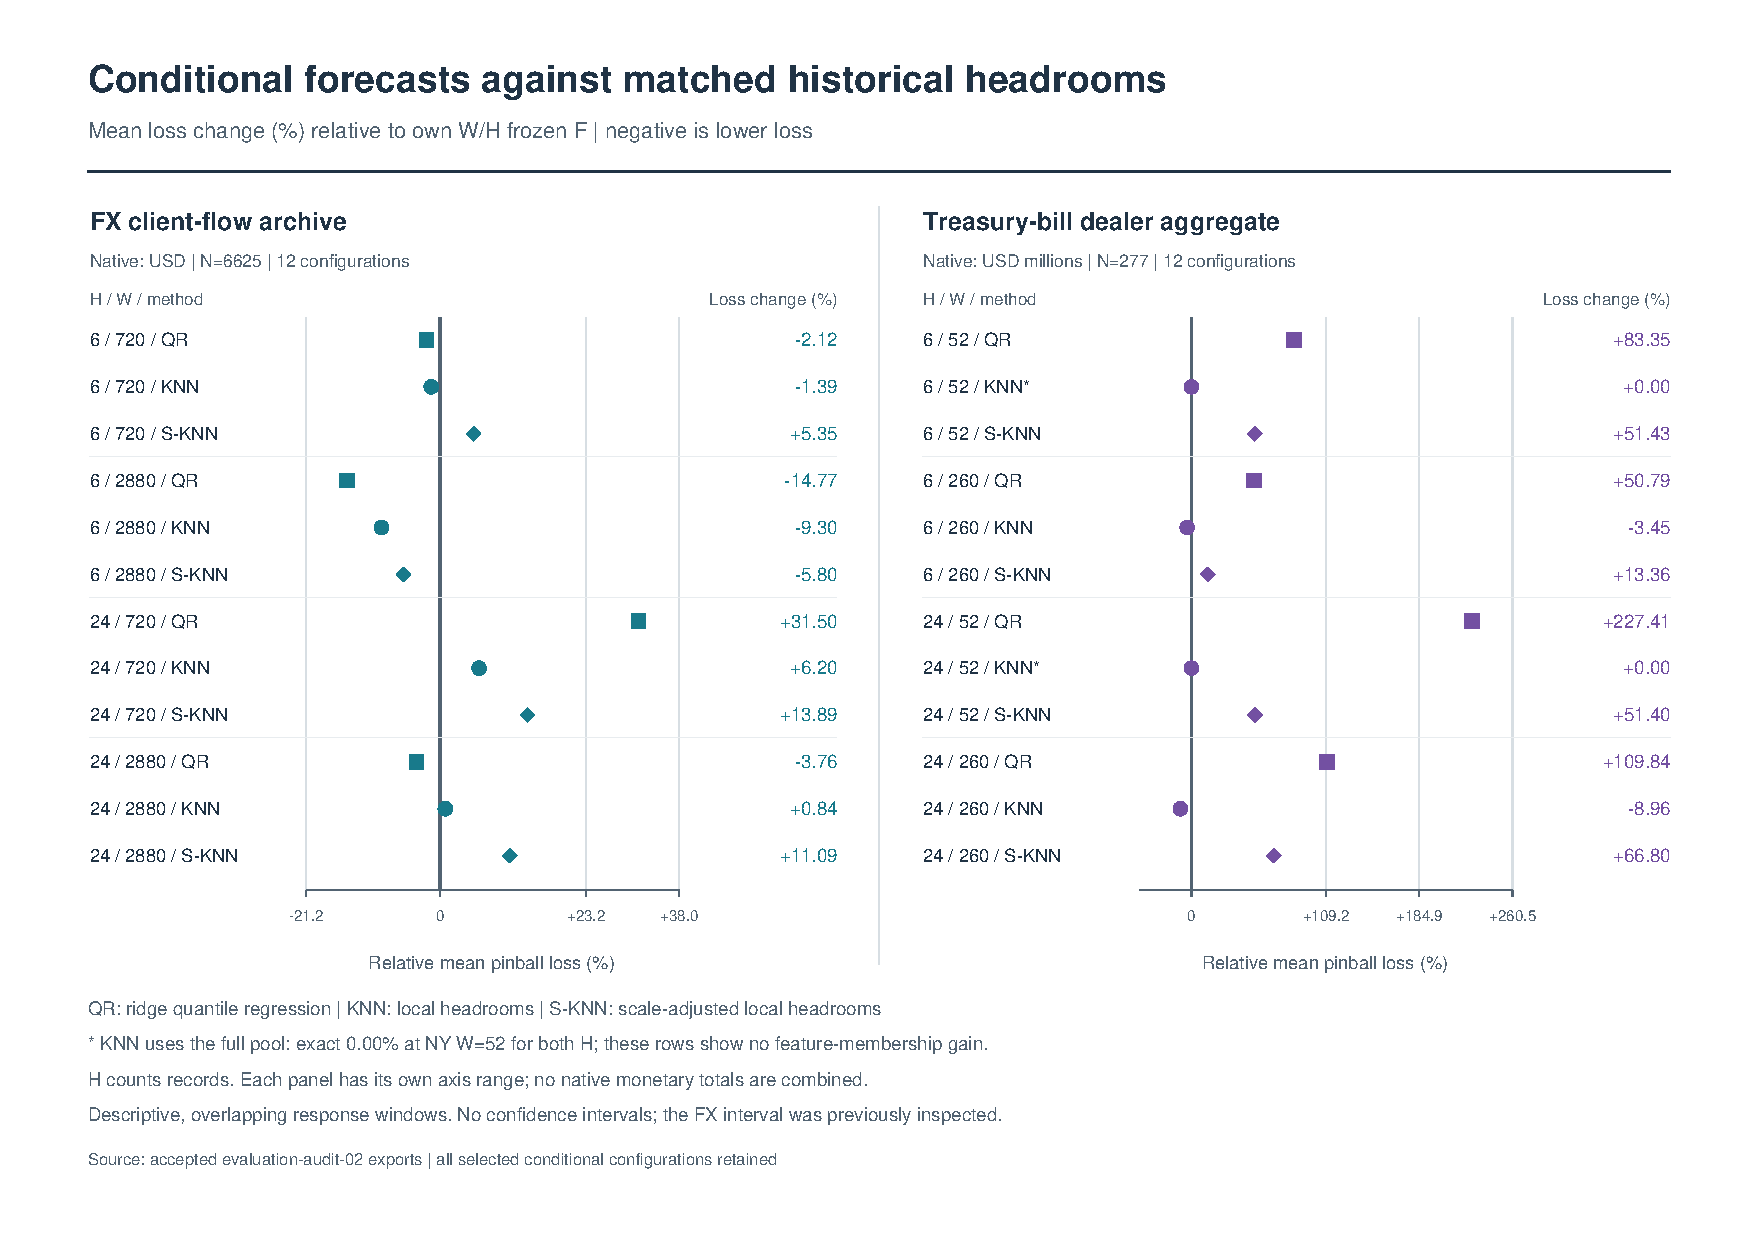
\includegraphics[width=\linewidth]{figures/conditional-common-history.pdf}
\par\smallskip
\small Figure 1. All 24 selected conditional forecasts versus frozen F with the same source, horizon, history window and refit schedule. Points show within-reference mean-loss percentages; negative favors the conditional procedure. Source panels have explicit scales and are not pooled. Full-pool KNN identities are marked. No sampling interval or conditional-coverage claim is shown.
\end{figure}
\clearpage
\begin{figure}[p]
\centering
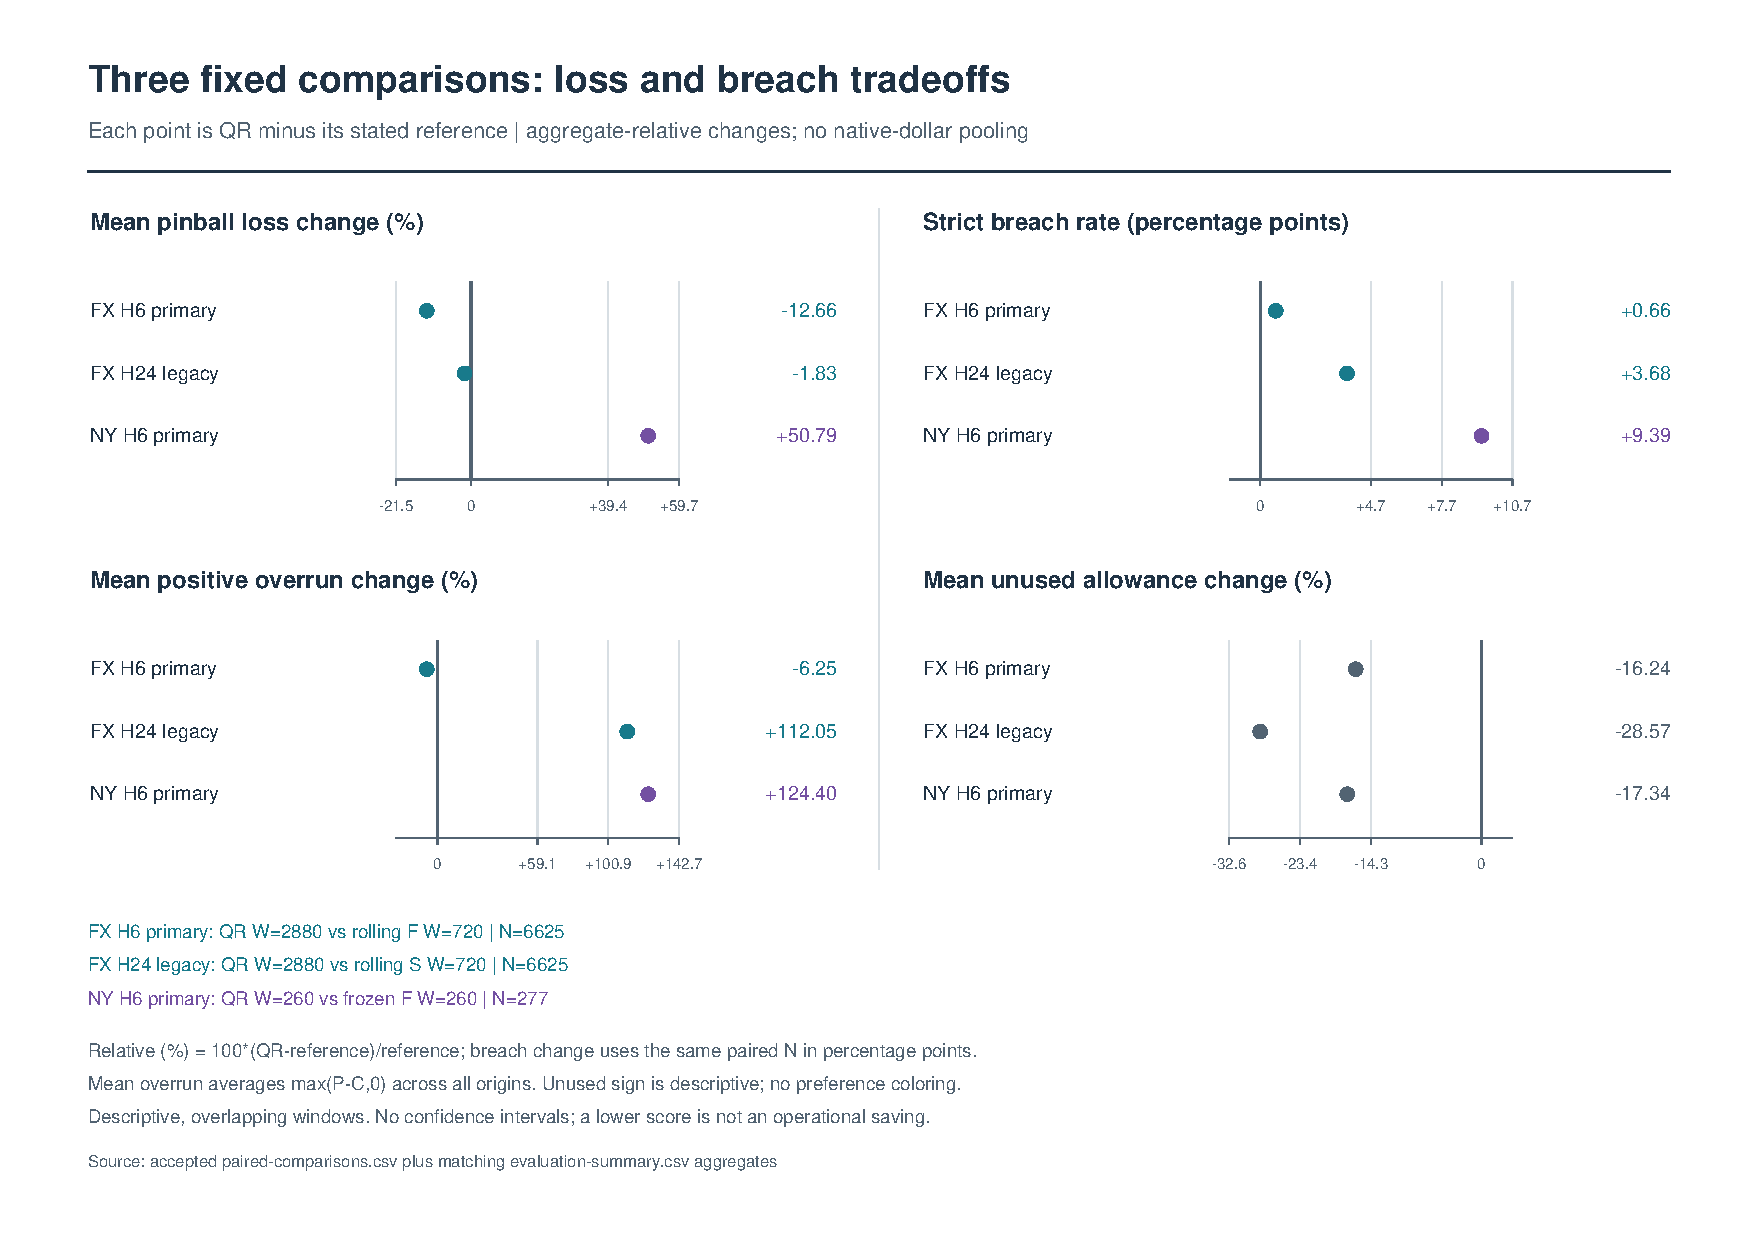
\includegraphics[width=\linewidth]{figures/conditional-primary-tradeoffs.pdf}
\par\smallskip
\small Figure 2. The two declared source primaries and FX H24 legacy-reference sensitivity: relative mean-loss, overrun and unused-allowance changes, plus breach-rate differences in percentage points. These are separate descriptive quantities, not a combined utility or monetary saving. A reduced unused quantity is not automatically overall improvement.
\end{figure}
\clearpage
\begin{figure}[p]
\centering
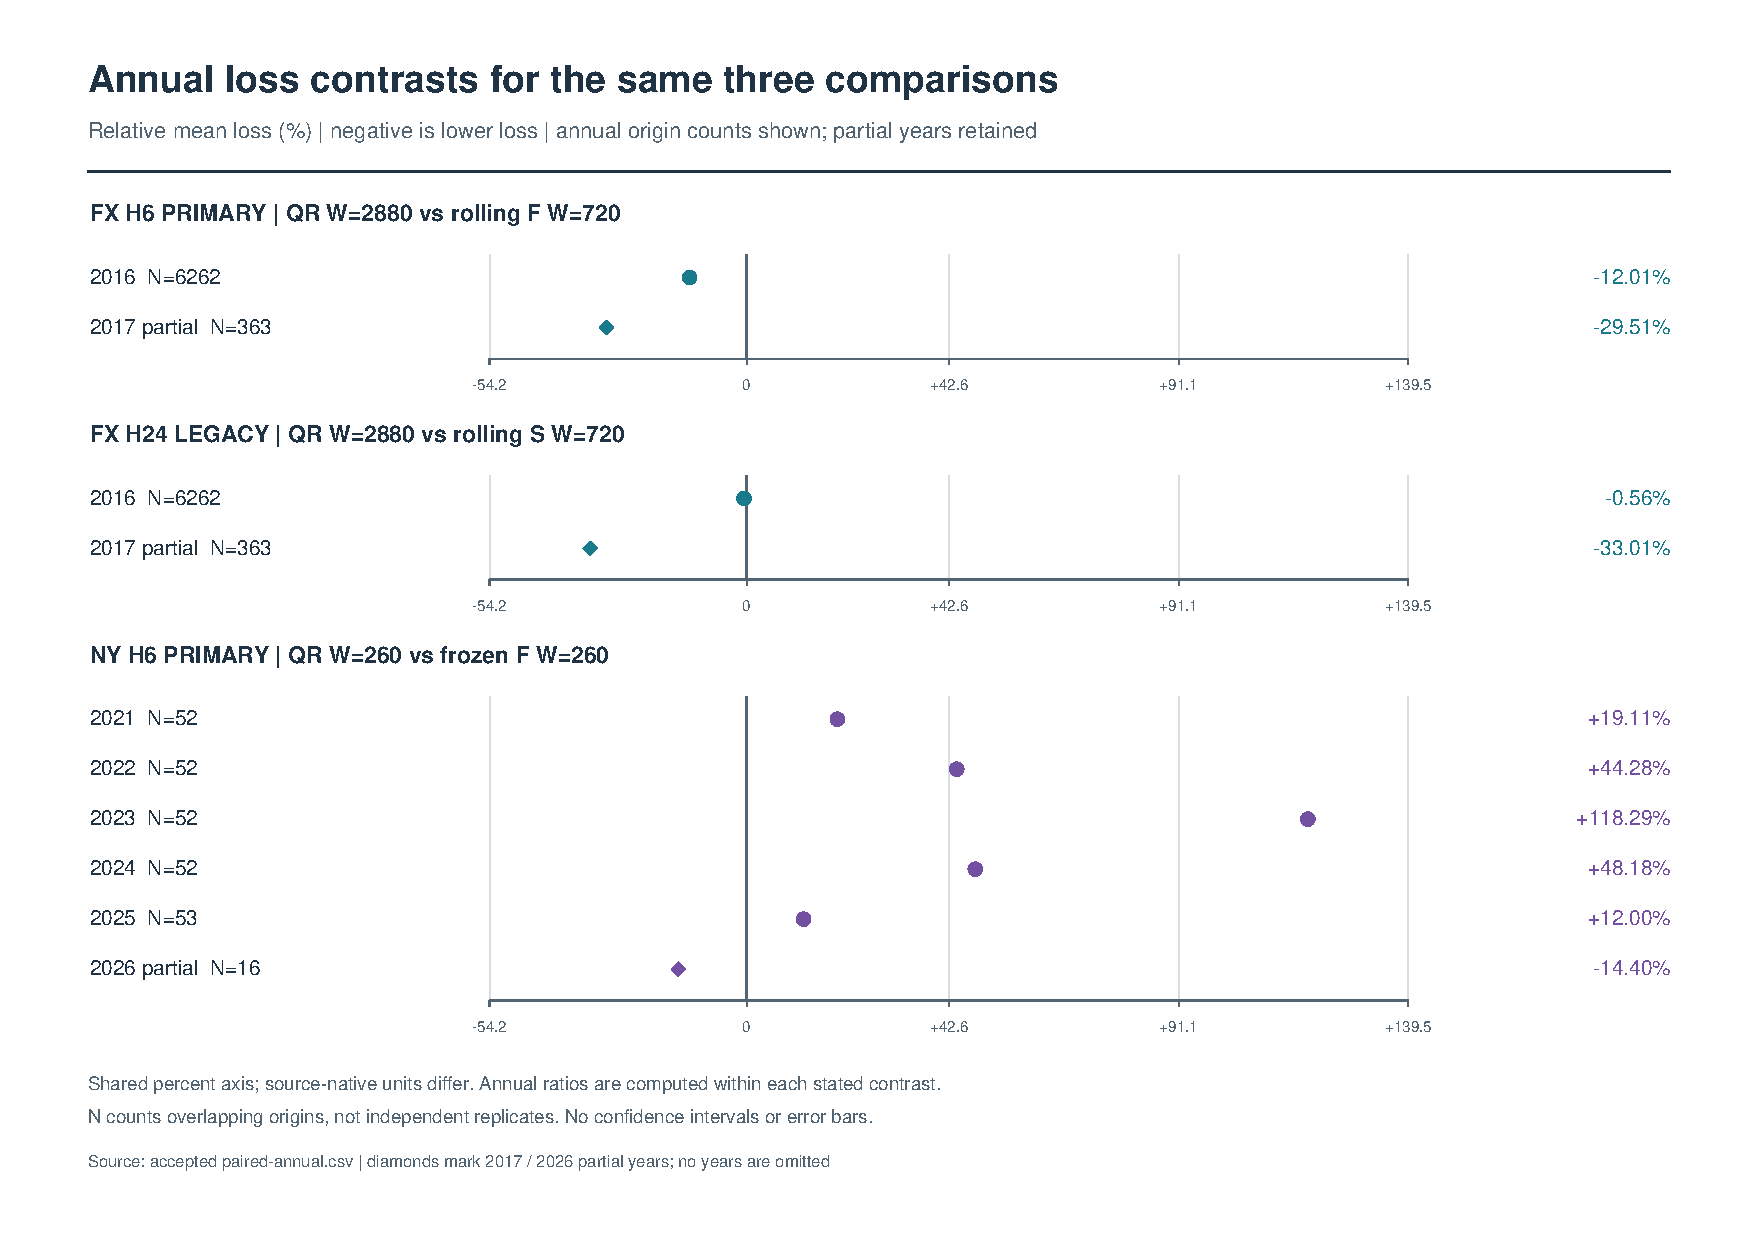
\includegraphics[width=\linewidth]{figures/conditional-annual-primary.pdf}
\par\smallskip
\small Figure 3. Every issue-year group for the two declared primaries and FX H24 legacy sensitivity. Values are paired within-reference loss percentages, with origin counts and partial years labeled. They are subdivisions of the same source records, not independent replications, confidence intervals or retrospectively selected switching regimes.
\end{figure}
\clearpage
\end{document}
